\documentclass[a4paper,12pt]{article}
\usepackage{latexsym}
\usepackage[polish]{babel}
\usepackage[utf8]{inputenc}
\usepackage[OT4]{fontenc}
\usepackage{fancyhdr}
\usepackage{amsmath}
\usepackage{amsthm}
\usepackage[pdftex]{graphicx}
\usepackage{graphicx}
\fancypagestyle{plain}{
% zmiana liter w~żywej paginie na małe
%\renewcommand{\chaptermark}[1]{\markboth{#1}{}}
%\renewcommand{\sectionmark}[1]{\markright{\thesection\ #1}}
\fancyhf{} % usuń bieżące ustawienia pagin
\fancyhead[LE,RO]{\date{\today}}
\fancyhead[LO]{Lokalne Sieci Komputerowe, laboratorium}
\renewcommand{\headrulewidth}{1.0pt}
\renewcommand{\footrulewidth}{1pt}
\addtolength{\headheight}{1.5pt} % pionowy odstęp na kreskę
\fancyfoot[LE,CO]{Michał Brzeziński-Spiczak, Krzysztof Dobosz}
\fancyfoot[LE,RO]{\thepage}
\renewcommand{\headrulewidth}{1pt} % pozioma kreska
}
%\addtolength{\textheight}{3.0cm}
%\addtolength{\hoffset}{-1.3cm}
%\addtolength{\textwidth}{2.7cm}
%\addtolength{\marginparwidth}{-2cm}
%\voffset = -50pt


\begin{document}
\pagestyle{plain}

\begin{titlepage}
 


 
% Upper part of the page
\flushleft{
\includegraphics[width=0.25\textwidth]{pwr}\\[1cm]
\textsc{Politechnika Wrocławska\\
Wydział Informatyki i Zarządzania\\
Kierunek: Informatyka\\
Rok: IV}}\\[1cm] 
 \begin{center}
%\textsc{\LARGE Lokalne Sieci Komputerowe\\Laboratorium}\\[1.5cm]
 
\textsc{ Sprawozdanie z ćwiczeń laboratoryjnych do przedmiotu LOKALNE
SIECI KOMPUTEROWE}\\[1.5cm]
 
 
% Title
 \hrule height 1pt
  \par
  \vfil \vskip 0.5cm
   
{ \large \bfseries GTT\\
GoogleMapsTimetable\\
Integracja rozkładu jazdy i Google Maps}\\[0.8cm]
 
  \hrule height 1pt
  \par
  \vfil \vskip 3.5cm

% Author and supervisor 
\begin{minipage}{0.55\textwidth}
\begin{flushleft} \large
\emph{Autorzy:}\\
Michał \textsc{Brzeziński-Spiczak}\\
Krzysztof \textsc{Dobosz}\\
\end{flushleft}
\end{minipage}
\begin{minipage}{0.4\textwidth}
\begin{flushright} \large
\emph{Prowadzący:} \\
dr inż. Ziemowit \textsc{Nowak}
\end{flushright}
\end{minipage}
 
\vfill
 
% Bottom of the page
{\large \today}
 
\end{center}
 
\end{titlepage}
\newpage
\tableofcontents
\newpage
%%%%%%właściwa treść:
\section*{Wprowadzenie} 


W miastach takich jaki Wrocław komunikacja miejska jest często najszybszą formą
transportu. Dla tych, którzy są w danym mieście przejazdem, w odwiedzinach --
często też jedyną. Problemem może jednak okazać się wówczas nie sama prędkość
autobusów czy tramwajów, ale czas jaki trzeba poświęcić na odnalezienie odpowiedniej linii, połączenia.

Najprostsze wyjście -- przygotować się. Rozkłady
jazdy są ogólno dostępne. W Internecie pojawia się coraz więcej portali
oferujących wyszukiwarki połączeń. Jednak i w taki przypadku pojawia się
problem -- trzeba wiedzieć między jakimi przystankami znaleźć połączenie. Zatem
jaki przystanek jest najbliżej miejsca, do którego muszę się dostać?

\textbf{GTT \emph{GoogleMapsTimetable}} proponuje rozwiązanie i tego problemu:
integracja rozkładów jazdy komunikacji miejskiej, wyszukiwarki połączeń oraz
map (bazując na znanym systemie \emph{GoogleMaps}).

Wykorzystanie planu miasta wprowadza nowe możliwości -- w najogólniejszym
przypadku wystarczy wyklikac na mapie punkt startowy, następnie punkt docelowy
i wcisnąć \emph{Szukaj}, aby dowiedzieć się jak (i gdzie konkretnie, czyli na
jaki przystanek) dojechać, żeby znaleźć się tam, gdzie jest to konieczne.

Nie jest to z pewnością pomysł innowacyjny. Można odnaleźć ślady i wzmianki
po wielu systemach mających na celu podobne udogodnienie korzystania z
rozkładów jazdy komunikacji miejskiej, jednak działających systemów jest nie
wiele. W trakcie prac nad powstaniem \textbf{GTT} swojej premiery doczekał się
portal \emph{jakdojade.pl}\footnote{www.jakdojade.pl}, o którym można
powiedzieć, że w głównej mierze spełnia stawiane wymagania.

\section{Analiza wymagań funkcjonalnych}
Głównym celem powstania aplikacji było ogólnie rozumiane zintegrowanie
rozkładów jazdy komunikacji miejskiej we Wrocławiu z systemem map serwisu
\emph{Google Maps}. Z tak postawionego celu wyrastają wymagania funkcjonalne:
\begin{enumerate}
  \item wyszukiwanie połączeń pomiędzy wybranymi punktami na terenie Wrocławia
  -- wybieranie odbywa się za pomocą wyszukiwarki lub poprzez kliknięcie na
  mapie;
  \item wizualizacja na mapie serwisu \emph{Google Maps}:
  \begin{itemize}
    \item przystanków,
    \item tras linii autobusowych/tramwajowych,
    \item połączeń wyszukanych przez użytkownika;
  \end{itemize}
  \item zautomatyzowanie aktualizacji rozkładów jazdy;
  \item przegląd tabliczek przystankowych (rozkładów odjazdów z zadanego
  przystanku).
  \item (\ldots)
\end{enumerate}
\section{Analiza dostępnych danych wejściowych systemu}
W systemie itegrującym ogólnodostępne dane konieczne jest zdefiniowanie i
odpowiednie przetwarzanie danych źródłowych. Wśród źródeł wymienić należy:
\begin{itemize}
  \item rozkład jazdy komunikacji miejskiej MPK Wrocław
  
  wstępna analiza wykazała dostępność rozkładów jazdy w postaci plików XML
  na stronach portalu Urzędu Miasta
  Wrocław\footnote{http://www.wroclaw.pl/m3298/p3714.aspx}
  \item lokalizacja (współrzędne geograficzne przystanków)

   podobnie udostępniane przez portal Urzędu Miasta w postaci plików
   ShapeFile\footnote{http://www.wroclaw.pl/m3293/}
  \item mapy 
  
  ze względu na wstępne wymagania projektowe spośród dostępnych dostawców map
  internetowych wybrano \emph{GoogleMaps} jeden z serwisów firmy \emph{Google},
  który z założenia ma być bazą danych map oraz zdjęć satelitarnych i
  lotniczych całego świata, a ponadto do którego zgodnie z zasadami działa
  firmy istnieje co najmniej kilka API pozwalających na wykorzystanie map we
  własnych serwisach.
\end{itemize}

Więcej informacji na temat sposobu przetwarzania danych wejściowych w kolejnych
sekcjach dokumentacji.

\section{Zarys zasady działania aplikacji}
Schematycznie zarys działa \textbf{GTT \emph{GoogleMapsTimetable}} przedstawia
diagram z Rys. \ref{dzialanie_systemu}. 

Aplikacja w momencie aktualizacji danych źródłowych pobiera z serwisu Urzędu
Miasta we Wrocławiu archiwum zawierające pliki XML z rozkładami jazdy
poszczególnych linii, jeżeli dane te są nowsze niż znajdujące się w wewnętrznej
bazie systemu (el. administracyjny). Po rozpakowaniu do katalogu tymczasowego
pliki te kolejno są parsowane, a dane z nich ładowane do bazy. Podobnie
wczytywane są z wcześniej przygotowanego pliku \emph{csv} współrzędne
geograficzne przystanków autobusowych i tramwajowych. Aktualizację/wypełnianie
danymi kończy utworzenie tabeli reprezentującej strukturę grafu połączeń między
przystankami, służącej później jako podstawa silnika wyszukiwania.

Dla użytkownika udostępnionych jest kilka scenariuszy zachowań, które można
dowolnie łączyć ze sobą:
\begin{itemize}
  \item wyszukiwanie połączeń punkt-punkty
  
  Za pomocą wyszukiwarki, bądź też poprzez kilknięcie na mapie wybierane są
  punkty: startu i docelowy. Po dobranio opcji wyszukiwania (ustaleniu typów
  linii) następuje uruchomienie silnika wyszukiwania. Silnik wyszukuje
  przystanki znajdujące się najbliżej punktu startowego i końcowego po
  czym  ładuje strukturę skierowanego multigrafu, w którym wyszukuje
  najkrótszych ścieżek względem kryterium najmniejszej liczby przesiadek
  wydobywająć najlepsze połączenia między przystankami. Operacja jest
  powtarzana dla kilku najbliższych przystanków, a lista wyników sortowana
 na podstawie liczby przesiadek oraz liczby pokonanych przestanków.
 
 Wyniki prezentowane są użytkownikowi m.in. w formie graficznej na mapie
 serwisu \emph{Google Maps}.
 \item wyszukiwanie przystanków
 
 Korzystając z wyszukiwarki przystanków użytkownik może odnaleźć przystanki
 odpowiadające wpisanej nazwie (fizycznie odbywa się to poprzez realizację
 zapytań do bazy danych); przystanki zostają naniesione na mapę.
 \item podgląd tras wybranych linii komunikacji miejskiej
 
 Po wpisaniu nazwy interesującej linii i wybraniu wariantu danej linii na mapę
 nanoszone są przystanki w kolejnosci pokonywania na trasie.
\end{itemize}

 \begin{figure}[htp]
\centering
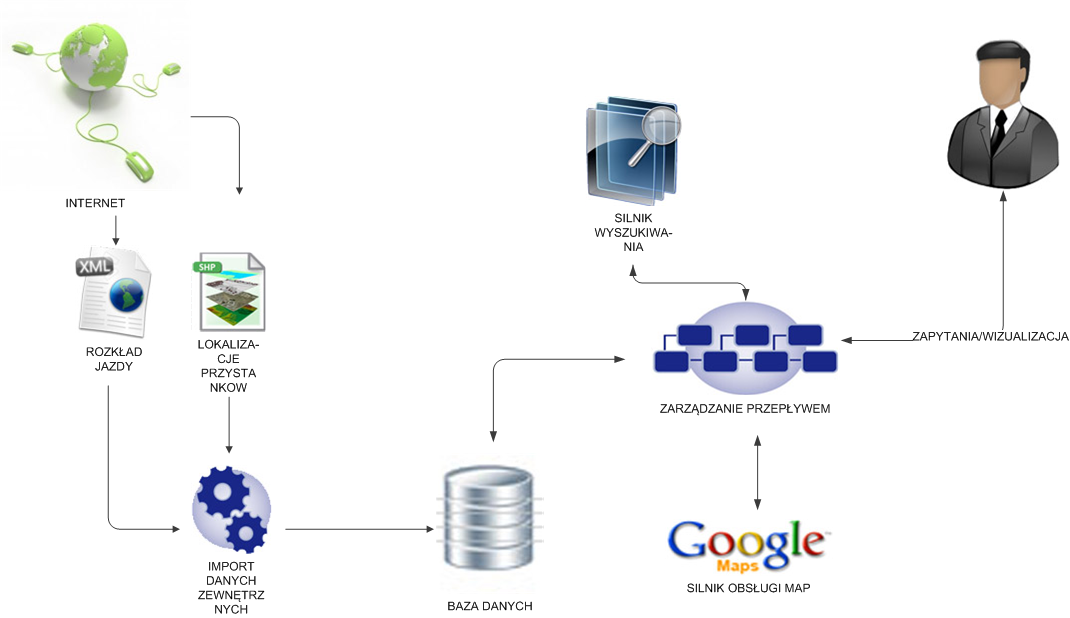
\includegraphics[width=\textwidth]{dzialanie_systemu} 
\caption{Zarys działania aplikacji -- diagram}\label{dzialanie_systemu}
\end{figure}

\section{Stosowane rozwiązania technologiczne}
\textbf{GTT \emph{GoogleMapsTimetable}} został napisany przy pomocy frameworka
GWT\footnote{http://code.google.com/intl/pl/webtoolkit/}. GWT oferuje możliwość
tworzenia serwisów javascriptowych bez konieczności pisania w tym uciążliwym
dla wielu programistów języku. Kod napisany w GWT bardzo przypomina kod w javie,
przez co cały framework można określic jako język java okrojony tak, żeby dało się
go skompilować do javascriptu.

Oprócz prostego tworzenia interfejsów użytkownika
GWT oferuje system komunikacji z częścią serwerową (napisaną w języku java) oparty
o RPC (Remote Procedure Call), będący w rzeczywistości tylko swego rodzaju warstwą
abstrakcji nad popularną komunikacją servletową. System ten charakteryzuje się tym,
że udostępnia komunikację asynchroniczną, aplikacja kliencka nie czeka na odpowiedź
z serwera, tylko wykonuje odpowiedni kod kiedy już ją dostanie.

Część serwerowa wykorzystuje również poza bibliotekami standardowymi:
\begin{itemize}
  \item \emph{JGrapht}\footnote{http://jgrapht.sourceforge.net/} -- bibliotekę
  udostępniająca metody obsługi oraz algorytmy przetwarzania grafów
\end{itemize}

Jako system zarządzania bazami danych wykorzystywany jest \emph{MySQL}, którego
obsługa dokonywana jest przy użyciu \emph{JDBC} -- niskopoziomowego interfejsu
wywołującego zapytania języka \emph{SQL}.

\section{Struktura systemu}

Opisywana aplikacja charakteryzuje się klasyczną strukturą webową typu
klient-serwer.

Na najwyższym poziomie ogólności przyjąć można, że część kliencka jest
interfejsem użytkownika: odpowiada za pobieranie danych wejściowych (zapytań do
systemu) oraz graficzną prezentację wyników działania systemu, natomiast część
serwerowa stanowi jądro realizujące zadania systemu.

Ze względu na fakt nałożenia znaczących wymagań funkcjonalnych odnośnie samego
interfejsu użytkownika część kliencka musi być traktowana na równi z serwerową.

\subsection{Część serwerowa}
Przyglądając się bliżej części serwerowej można wyodrębnić następujące moduły
funkcjonalne aplikacji:
\begin{itemize}
  \item zarządzanie bazą danych;
  \item zarządzanie pozyskiwaniem danych z zewnętrznych źródeł;
  \item silnik wyszukiwania połączeń;
  \item zarządzanie komunikacją z częścią kliencką
\end{itemize}
\subsubsection{Zarządzanie bazą danych}
Moduł zarządznia bazą danych stanowi łącznik między warstwą danych a
pozostałymi modułami serwera i pośrednio częścią kliencką. Jest najniższą
warstwą abstrakcji nałożoną na fizyczną realizację systemu zarządzania bazą
danych. 

Po analizie struktury danych źródłowych opracowano strukturę bazy danych
stanowiącej źródło danych dla całego systemu. Strukturę przedstawiono na Rys.
\ref{schemat_bazy_danych}

 \begin{figure}[htp]
\centering
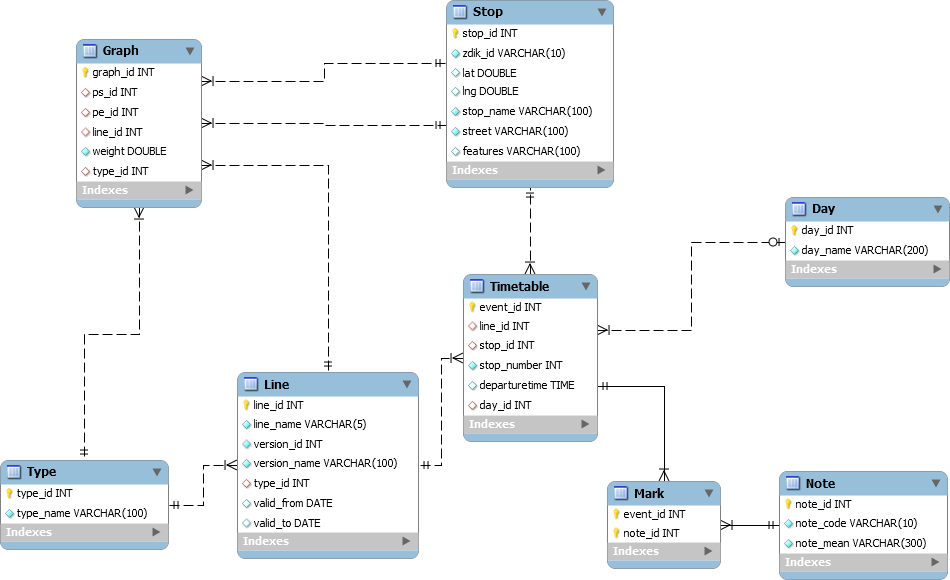
\includegraphics[width=0.8\textwidth]{schemat_bazy_danych} 
\caption{Diagram ER bazy danych}\label{schemat_bazy_danych}
\end{figure}

W strukturze tej wyodrębnić należy tebele:
\begin{enumerate}
  \item STOP -- zawiera kompletne informacje o przystankach zarówno
  autobusowych jak i tramwajowych; wśród nich:
  \begin{itemize}
    \item zdik\_id -- identyfikator przystanku wg MPK Wrocław
    \item lat, lng -- współrzędne geograficzne przystanku
    \item stop\_name -- nazwa przystanku
    \item street -- ulica
    \item features -- cechy dodatkowe (występują w źródłach rozkładów,
    aktualnie niewykorzystywane w systemie)
  \end{itemize}
  \item DAY -- wyodrębnione typy dni, w których występują zmiany kursowania
  komunikacji miejskiej.
  \item LINE -- aktualnie kursujące linie autobusowe i tramwajowe:
  \begin{itemize}
    \item line\_name -- nazwa lini
    \item version\_name -- nazwa wariantu (również zjadu do zajezdni itp.)
    \item valid\_from, valid\_to -- czas, w którym rozkłady utrzymują ważność
    \item type\_id -- klucz do typu linii 
  \end{itemize}
  \item TYPE -- informacje o typach linii (normalne, pospieszne, różne rodzaje
  typów nocnych)
  \item TIMETABLE -- tabela zbiorcza przechowyjąca dane o czasach odjazdów
  pojazdu danej linii z danego przystanku
  \item NOTE -- zgrupowane przypisy (np. N - autobus niskopodłogowy)
  \item MARK -- tabela reprezentująca relacje wiele-do-wielu przypisująca
  przypisy do zadanego kursu (dokładniej -- zdarzenia zatrzymania pojazdu na
  przystanku) 
  \item GRAPH -- tabela wprowadzona ze względów optymalizacyjnych
  przechowywująca strukturę grafu połączeń między przystankami.
\end{enumerate}
 
 Moduł zarządzania bazą danych udostępnia metody wyodrębniające dane potrzebne
 do prawidłowego funkcjonowania pozostałych modułów.
 
\subsubsection{Pozyskiwaniem danych z zewnętrznych źródeł}
Moduł ten odpowiada za pobieranie i przetwarzanie danych z zewnętrznych źródeł
do postaci możliwej do zapisania w bazie danych. Realizuje weryfikację
konieczności aktualizacji (sprawdzenie czy dane w portalu UM Wrocław są nowsze
niż przechowywane w bazie wewnętrznej systemu), pobieranie archiwów,
wypakowywanie plików, parsowanie plików XML i zapisywanie wyodrębionych danych
do bazy.
 

\subsubsection{Silnik wyszukiwania połączeń}
Na podstawie relacyjnej struktury danych moduł ma za zadanie generowanie
najlepszych połączeń między zadanymi punktami.

Pierwszym elementem działania jest odnalezienie przystanków najbliższych
zadanemu punktowi startowemu i końcowemu na podstawie współrzędnych
geograficznych. Następnie ma miejsce właściwe wyszukiwanie połączeń
przystanek-przystanek.

W tym celu wykorzystywana jest struktura ważonego multigrafu skierowanego.
Wierzchołki grafu reprezentują przystanki,  krawędzie -- występowanie
bezpośredniego (bezprzesiadkowego) połączenia miedzy przystankami. Dodatkowo
krawędzie występują w przypadku przystanków o tej samej nazwie (węzły
komunikacyjne) z wagą równą odległości (w kilometrach) między tymi
przystankami, jeśli odległość ta jest nie większa niz $400$m. 

Na tak zbudowanej strukturze wywoływany jest algorytm \emph{k-shortest paths}
wyszukujący $k$ najkrótszych ścieżek między zadanymi wierzchołkami. W
implementacji jest to połączenie algorytmów Dijkstry oraz
Bellmana-Forda; samej metody wyszukiwania dostarcza biblioteka \emph{JGrapht}.

Rezultaty wyszukiwania dla każdej pary najbliższych przystanków zadanym punktom
są łączone minimalizując kryteria: najpierw liczby przesiadek, następnie
odległości przystankowej (sumie liczby przejechanych przystanków).


\subsubsection{Komunikacja z częścią kliencką}
 Wymaganą funkcjonalność w operowaniu na zbiorach bazy danych zapewniają
 udostępnione metody modułu Zarządzania bazą danych. Samą komunikacją między
 częścią serwerową a klienckę zdecydowano obarczyć framework \emph{GWT}, na
 temat którego więcej informacji w sekcji Stosowanych rozwiązań technologicznych.

\subsection{Część kliencka}
 Moduły funkcjonalne jakie można wyróżnić w aplikacji klienckiej to:
\begin{itemize}
\item część wizualna interfejsu
\item część funkcjonalna interfejsu
\item interfejsy komunikacji z serwerem
\end{itemize}

\subsubsection{GUI}
Graficzny interfejs użytkownika jest w wysokim stopniu intuicyjny. Opiera się
głównie na klasie \emph{GWT} AbsolutePanel, dzięki której tworzenie interfejsu przypomina
układanie warstw, podobnie jak w języku \emph{HTML}. Największym widgetem jaki użytkownik
widzi na stronie jest oczywiście mapa, której wygląd zależy w dużej mierze od tego
co udostępniła firma \emph{Google} w swoim API do \emph{GWT}. Pola tekstowe, przyciski, itp.
zostały umieszczone w stronie na stałe, tzn. nie przesuwają się przy zmianie
rozmiaru strony. Większość z ich to obiekty klas udostępnionych przez framework,
własnym wkładem natomiast są wszelkie obrazki i ikonki (także tło). Także ikonki
markerów na mapie są pobierane ze strony \emph{GoogleMaps}. Więcej o interfejsie
w Podręczniku Użytkownika. Cała graficzna część interfejsu użytkownika znajduje się
w klasie Client.java.

\subsection{Funkcjonalność interfejsu}
Oprócz oczywistej funkcjonalności, takiej jak odczytywanie ciągów znaków z
odpowiednich pól, czy obsługiwanie zdarzeń takich jak wciśnięcie przycisku,
najbardziej istotne funkcje spełniają markery nanoszone na mapę. To z ich
pomocą użytkownik decyduje o punktach początkowych i końcowych trasy, także
to one reprezentują znalezione przystanki. System obsługujący markery jest
dość skomplikowany, musi reagować odpowiednio na zmianę punktu początkowego
trasy, dodawać i usuwać w markery w odpowiednim czasie. W celu lepszego
przypisania dymków, które zawierają linki do wszystkich funkji ,do markerów,
stworzono klasę GttMarker dziedziczącą po klasie Marker. Zaszła również
konieczność stworzenia kontenera na dane potrzebne do prawidłowego pokazania
rozkładu odjazdów danej linii z danego przystanku, ponieważ mimo asynchronicznej
komunikacji do wyświetlenia rozkładu potrzebne są wszystkie dane. Moduł
funkcjonalności obejmuje klasy Client.java, TimetableData.java oraz GttMarker.java.

\subsection{Interfejsy komunikacji z serwerem}
System komunikacji oparty o RPC wymaga od developera stworzenia dwóch interfejsów
dla każdej usługi - jeden synchroniczny, drugi asynchroniczny. Komunikacja
odbywa się przez drugi interfejs. Po stronie serwera musi istnieć skompilowana
klasa implementująca synchroniczny interfejs.

\subsection{Model obiektowy systemu}
Oczywiście ogólnie system stworzony został w oparciu o paradygmat obiektowości.
Część serwerowa została napisana w języku java, a część kliencka we frameworku GWT,
które to języki programowani są językami czysto obiektowymi. 

\subsubsection{Diagram klas}

Diagram klas przedstawia rysunek \ref{diagram_klas}.

 \begin{figure}[htp]
\centering
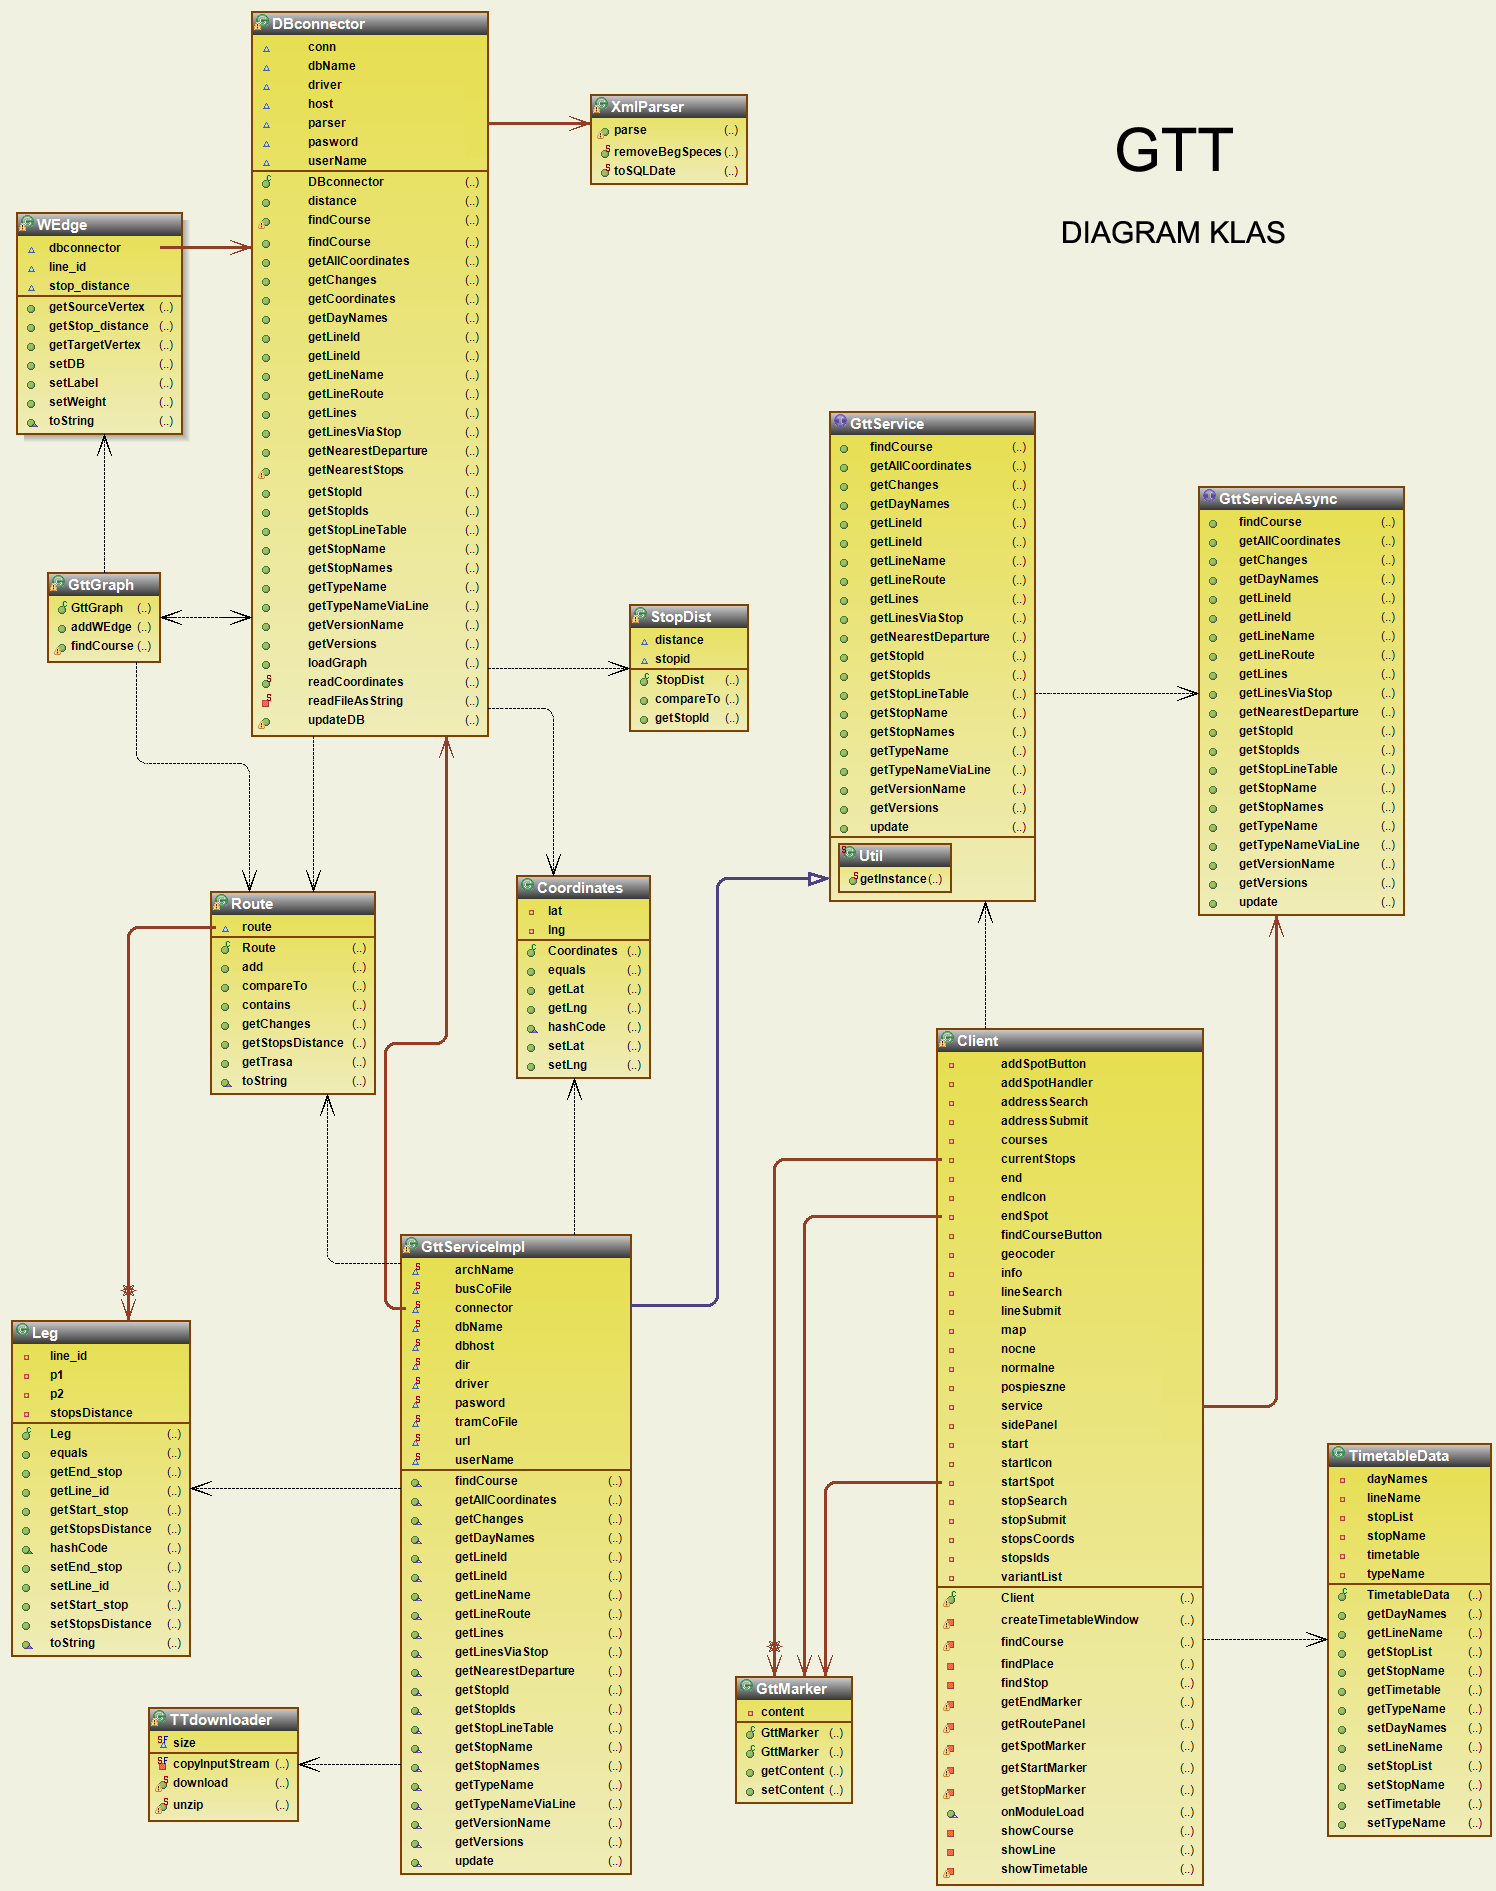
\includegraphics[width=\textwidth]{diagram_klas} 
\caption{\textbf{GTT} -- Diagram klas}\label{diagram_klas}
\end{figure}
\section{Specyfikacja środowiska działania}

\section{Plany rozwojowe} 

 \textbf{GTT \emph{GoogleMapsTimetable}} w aktualnej formie realizuje nałożone
 wymagania funkcjonalne jednak podczas prac nad jego tworzeniem pojawiły się
 nowe pomysły jak i problemy, co do których warto odnaleźć lepsze rozwiązania
 niż obecnie zastosowane.
 
 Zarys planów rozwojowych:
 
 \begin{itemize}
   \item automatyzacja importu lokalizacji przystanków z zewnętrznych źródeł;
   \item poprawa wydajności aktualizacji rozkładów;
   \item poprawa wydajności i funkcjonalności silnika wyszukiwania połączeń
   (własna implementacja biblioteki do obsługi grafów dopuszczająca
   wielopoziomowe kryteria jakości wyszukiwania najkrótszych ścieżek);
   \item wyszukiwania połączeń z punktami pośrednimi;
   \item uogólnienie schematy w celu zastosowania również dla innych miast niż
   Wrocław;
   \item wprowadzenie panelu administracyjnego umożliwiającego ręczną
   modyfikację pól bazy danych (głównie lokalizacja przystanków, ze względu na
   wystepujące problemy);
   \item dołożenie funkcjonalności wyszukiwania z wykorzystaniem
   kryterium czasowego (problematyczne ze względu na brak deterministycznej
   metody określania czasu przejazdu przystanek-przystanek na podstawie posiadanych rozkładów)
   \item \ldots
 \end{itemize}

\section{Raport z realizacji części serwerowej}
Prace nad częścią serwerową rozpoczęły się równolegle do przyswajania i
zaaklimatyzowania się z \emph{GWT Google Maps API}. Ustalona została logiczna
kolejność funkcjonalna tworzenia klas i realizacji modułów funkcjonalnych:
\begin{itemize}
  \item analiza struktury dokumentów XML z rozkładami jazdy 
  \item opracowanie struktury bazy danych
  \item programowe pozyskanie dokumentów XML z rozkładami
  \item wyodrębnienie interesujących danych -- parsowanie
  \item wypełnienie bazy danych
  \item opracowanie silnika wyszukiwania połączeń
  \item zdefiniowanie i oprogramowanie interfejsów pobierania informacji o
  rozkładach
  \item opracowanie interfejsów silnika wyszukiwania połączeń
  \item implementacja silnika wyszukiwania połączeń przystanek-przystanek
  \item analiza struktury i możliwości importu lokalizacji przystanków z plików
  źródłowych
  \item aktualizacja bazy danych o lokalizację przystanków 
  \item implementacja silnika wyszukiwania połączęń punkt-punkt 
\end{itemize}

  \subsection{Pozyskiwanie i wczytywanie danych z zewnętrznych źródeł }
  Pozyskane z portalu Urzędy Miasta we Wrocławiu pliki XML zawierające rozkłady
  jazdy dla poszczególnych linii wydawały się początkowo dobrze zorganizowane i
  spójne. Schemat XML oraz wyobrażenie funkcjonowania systemu pozwoliły w dość
  jasny sposób zbudować strukturę bazy danych, która nie uległa większym zmianom
  aż do uzyskania funkcjonującej wersji aplikacji oraz przygotować parser w
  celu wypełnienia danych. Problemy pojawiły się jednak przy próbnych
  ładowaniach. Występowały niespójności nie tyle na poziomie schematu co samych
  danych. Pojawiały się losowo białe znaki w nazwach linii czy tym bardziej
  oznaczeniach, zdublowane godziny odjazdów (z których część okazała się nie
  stanowić błędu, a jedynie nieoczekiwaną rzeczywistość, zdecydowano jednak
  zignorować powtarzające się odjazdy o tej samej godzinie jako nie mające
  wpływu na proces wyszukiwania połączeń), zwielokrotnione oznaczenia (,,NN''
  oznaczające, że kurs jest realizowany przez autobus niskopodłogowy oraz
  że\ldots kurs jest realizowany przez autobus niskopodłogowy). Jeszcze
  bardziej uciążliwe było to, że niespójność ta ujawniała się systematycznie w
  trakcie prac wraz z aktualizacją danych, co zmuszało do poprawiania
  elementów parsera. 
  Dopiero po implementacji parsera rozpoczęły się prace nad  klasą
  TTDownloader odpowiedzialną za pobieranie archiwum rozkładów i jego
  wypakowywaniem, które po z literatury i dokumentacji języka okazały się
  bezproblemowe.
  Kłopotliwy pozostaje czas wczytywania danych do bazy sięgający 25 minut
  (czas ten jest większy w przypadku uruchamiania w systemi Windows ze
  względu na mniejszą wydajność maszyny wirtualnej Javy), jednak ze względu na
  to, że zmienność rozkładów jest stosunkowo nie wielka prace nad
  przyspieszeniem importu danych zostały odłożone do planów rozwojowych
  aplikacji. Przypuszczalnie poprawę przyniosłoby wstępne operowanie na
  strukturach danych języka przechowując w postaci np. list kolejne rekordy
  tabel a dopiero później zapisując je hurtowo do bazy w przeciwieństwie do
  rozdrobnionych operacji ładowania w aktualnej wersji; niewiadomą pozostaje
  jednak zużycie pamięci (sama tabela TIMETABLE zawiera blisko milion
  rekordów) -- czy nie spowoduje błędy typu \emph{out.of.memory}, co zmuszałoby
  to porcjowania danych np. w plikach.
  
  Znacznie później dodano metody pozwalające na aktualizację bazy danych o
  współrzędne geograficzne przystanków. 
  
  Dane takie podobnie jak rozkłady znajdują się na stronach portalu Urzędy
  Miasta we Wrocławiu w formie plików \emph{ShapeFile}. Ze wgzlędu na problemy
  z uruchomieniem dostępnych bibliotek obsługujących ten format zdecydowano o
  zastosowaniu wstępnej konwersji zewnętrzną aplikacją: \emph{DNR Garmin
  Application}\footnote{http://www.dnr.state.mn.us/mis/gis/tools/arcview/extensions/DNRGarmin/DNRGarmin.html}
  do formatu csv zawierającego wprost lokalizację -- współrzędne przystanków
  względem identyfikatora stosowanego przez MPK (zdikid). Pliki te dodane są na
  stałe do programu. Ze względu na to, że lokalizacja słupków przystankowych
  ulega zmianie niezwykle rzadko nie pobieranie i niewyodrębnianie tych danych
  przy każdej aktualizacji można uznać za zabieg optymalizacyjny. 
  
  Konwersja nie ustrzegła jednak przed problemami. Po aktualizacji bazy 51
  przystanków nie uzyskało informacji o lokalizacji. Ręczna analiza zarówna
  bazy danych (a zatem plików XML) jak i zawartości plików SHP pokazała, że w
  przypadku części z tych brakujących przystanków przekłamaniu uległ
  identyfikator -- numer słupka przystankowego (najczęściej jest to
  różnica/brak pierwszej cyfry). Część danych została uzupełniona ręcznie.
  \subsection{Silnik wyszukiwania połączeń}
  Projektowanie silnika wyszukiwania połączeń było najdłuższą fazą w trakcie
  prac analitycznych nad projektem. Początkowo starano się wyprowadzić własny
  algorytm wyszkiwania bazujący bezpośrednio na tabeli TIMETABLE. Próby jednak
  kończyły się bez wymiernych rezultatów najczęściej błedami metody lub
  też\ldots wyczerpaniem pamięci maszyny wirtualnej.
  Zdecydowano zatem przeformułować problem znajdowania połaczeń w komunikacji
  miejskiej na problem wyszukiwania najkrótszych ścieżek w grafie. W tym celu
  skorzystano z bilioteki \emph{JGraphT}. W dalszym ciągu pozostawało problemem
  zdefiniowanie wag połączeń oraz interpretacji co reprezentuje krawędź w
  grafie. Początkowo krawędzie reprezentowały połaczenia przystanków na
  zasadzie możliwości przejechania jedną linią bez przystanku pośredniego.
  Generowało to stosunkowo niewielką liczbę krawędzi (problem optymalizacyjny
  -- algorytm wyszukiwania k najkrótszych ścieżek charakteryzuje złożoność
  rzędy $O(k*m*n)$ gdzie $m$ to liczba krawędzi, a $n$ to liczba wierzchołków.
  O ile liczbą wierzchołków nie można było manipulować (w minimalnym stopniu
  udało się zrealizować to później) o tyle odpowiednia interpretacja krawędzi
  pozwalała na ograniczenie liczby $m$. Wyszukiwanie w takim przypadku co
  prawda odbywało się szybko, jednak pojawiały się wyniki akceptujące
  systematyczne przesiadki z jednej linii na drugą, gdyż takie również
  minimalizowały koszt wyrażony w odległości przystankowej. Do porcji
  eksperymentów wprowadzono zwieloktronienie krawędzi za sprawą zmiany
  interpretacji ich występowania: krawędź łączy dwa wierzchołki (przystanki)
  jeśli istnieje między nimi połączenie nie wymagające przesiadki. W ten sposób
  można było posłóżyć się wagą wyrażającą ilość przesiadek, jakich trzeba
  dokonać, aby dostać się z jednego przystanku na inny, kosztem czasu
  realizacji zapytania.
  
  Problem czasu wyszukiwania okazał się nie być jedynym. Realizacja zapytań do
  bazy danych pochłaniała go jeszcze więcej. Podjęto zatem próbę minimalizacji
  liczby zapytań do bazy poprzez utworzenie oddzielnej tabeli GRAPH
  przechowującej pełną strukturę grafu. Wczytywanie jej wymaga w tym momencie
  realizacji jednego zapytania do bazy. 
  
  W dalszym ciągu takie wyszukiwanie obsługiwało jedynie znajdowanie połączeń
  przystanek-przystanek bez możliwości przejścia pieszego między przystankami.
  Owocowało to bardzo częstymi wydłużonymi trasami w przypadku kiedy w
  rzeczywistości wystarczyłoby przejść na drugą stronę ulicy, na przystanek o
  tej samej nazwie, w tym samym węźle komunikacyjnym. Określając koszt takiego
  przejścia jako nieznaczący uzyskano możliwość przechodzenia między
  najbliższymi przystankami, jednak pojawiały się bezkosztowe krążenia między
  takimi przystankami. Konieczne było zatem wprowadzenie wagi. Ustalono, że
  przechodzić można na przystanek o tej samej nazwie tylko wówczas, jeżeli jest
  on bliżej niż 200m z wagą równej odleglości w kilometrach (waga krawędzi
  stanowiącej połączenie bez przesiadek wynosi 1).
  
  Ograniczenie ilości krawędzi w najczęstszych przypadkach wyszukiwania
  przyniosło sparametryzowanie metody wyszukiwania typami linii (tak, aby np.
  nie wyszukiwać połączeń liniami nocnymi w dzień) oraz ograniczenie
  wczytywania połączeń do grafu jedynie do dwóch podstawowych wariantów linii.
  
  Aby umożliwić wyszukiwanie połączeń między zadanymi punktami, niekoniecznie
  przystankami zdecydowano posłużyć się metodą wyszukiwania połączen
  przystanek-przystanek dla każdej pary przystanków spośród $p$ najbliższych
  zadanym punktom. Wyniki są następnie łącząne względem dwóch kryteriów -- wagi
  wyrażającej ilość przystanów oraz dodatkowej wagi określającej odległość
  przystankową.
  
  \subsection{Interfejsy komunikacji}
  W celu możliwości realizacji funkcjonalności części serwerowej na zapytania
  pochodzące od użytkownika opracowano i zaimplementowano szereg metod
  dostępowych do danych oraz struktury ich przekazywania. Opierają się one w
  głównej mierze na kombinacji struktur wbudowanych -- list i tablic
  hashujących. 

\section{Raport z realizacji części klienckiej}
Aplikacja kliencka powstawała w środowisku programistycznym Eclipse z dodatkiem
do obsługi projektów \emph{GWT} - Cypal Studio. Jako, że część developerów była
już zaznajomiona z frameworkiem \emph{GWT}, prace nad częścią kliencką rozpoczęły
się od importu i aplikacji do programu modułu \emph{GoogleMaps}. \emph{GWT} pozwala
na uruchamianie projektów w specjalnie przygotowanym do tego środowisku: wbudowanym
serwerze \emph{Tomcat} i prostej przeglądarce obsługującej javascript. Mimo to
doświadczenie podpowiadało, żeby przygotować skryptu kompilujące i uruchamiające
aplikację na zewnętrznym serwerze, ponieważ istnieją pewnie niezgodności między tym
co widzi developer na wbudowanej przeglądarce, a tym co widzi użytkownik po
uruchomieniu aplikacji w docelowym środowisku.

\subsection{System Markerów}
Po zaznajomieniu się z API do \emph{GoogleMaps} powstał pomysł, żeby dużą część
funkcjonalności serwisu oprzeć na Markerach. Omawiane API dysponuje dosyć dużą
liczbą czynności jakie można robić z Markerami, jednak nie ma tego co okazało się
bardzo potrzebne: przypisania Markerowi zawartości dymka który pokazuje sie po
kliknięciu na dany Marker. Tak powstała klasa GttMarker dziedzicząca po Markerze
z \emph{GWT}. Funkcjonalność Markerów zawiera m. in. odczyt współrzędnych
geograficznych z każdego punktu na mapie, oznaczenia Markerów jako początku lub
końca trasy, reprezentacja przystanków razem z liniami odwiedzającymi go, oraz
wyświetlaniem rozkładu jazdy itd.

\subsection{Prezentacja wyników}
Kolejną rozbudowaną częścią funkcjonalności jest prezentacja wyników wyszukiwania.
\textbf{GTT \emph{GoogleMapsTimetable}} pozwala na wyszukiwanie:
\begin{itemize}
\item przystanków o danej nazwie
\item wszystkich przystanków na trasie jednej, danej linii
\item połączeń między dwoma dowolnymi punktami w mieście
\end{itemize}
W pierwszym oraz drugim przypadku wyniki pokazują się w prostej liście na panelu bocznym.
Prezentacja wyników różnych tras na raz jakkolwiek okazała się nie być rzecza prostą.
Konieczne było przebudowanie sposobu wyświetlania wyników. Wcześniej przystanki dodawane
były do panelu bocznego w funkcji getStopMarker(), czyli podczas wyświetlania ich na mapie.
Podczas przebudowywania powstała funkcja getRoutePanel(), która tworzy pionową listę
z nazwami przystanków, a programista sam może zadecydować, czy po prostu pokazać tą listę
(dwa pierwsze przypadki), czy dodać ją do większej listy, uwzględniającej różne trasy
(trzeci przypadek).

\section{Podręcznik administratora}
Portal \textbf{GTT \emph{GoogleMapsTimetable}} stworzony został z myślą o tym,
że będzie on uruchamiany na serwerach typu \emph{Apache-Tomcat}. Do uruchomienia
aplikacji na domyślnych ustawieniach serwera wystarczy zamiania ścieżek do
folderu serwera, oraz do folderu z plikami jar \emph{GWT} oraz modułu \emph{GoogleMaps}
do \emph{GWT} w pliku \texttt{exports.sh}, oraz uruchomieniu skryptu budującego i
uruchamiającego całą aplikację \texttt{build.sh}. Skryptu zostały przygotowane
dla środowiska Linux.

\section{Podręcznik użytkownika}

 \textbf{GTT \emph{GoogleMapsTimetable}} jest webową aplikacją stanowiącą
 połaczenie rozkładów jazdy komunikacji miejskiej z systemem \emph{Google
 Maps}. Głównym celem programu jest umożliwienie intuicyjnego wyszukiwania
 połaczeń liniami komunikacji miejskiej między zadanymi punktami terenowymi w
 mieście. 
 
 Jedynym co jest wymagane do korzystania z systemu \textbf{GTT} jest
 przeglądarka internetowa z włączoną obsługą Java Script (standard) oraz
 połączenie do Internetu. Wystarczy w przeglądarce wpisać adres (\ldots).

 \textbf{GTT} charakteryzuje się prostym, funkcjonalnym interfejsem
 użytkownika przedstawionym na Rys. \ref{interfejs_help}, który składa się z 6
 głównych paneli funkcjonalnych:
  \begin{figure}[htp]
\centering
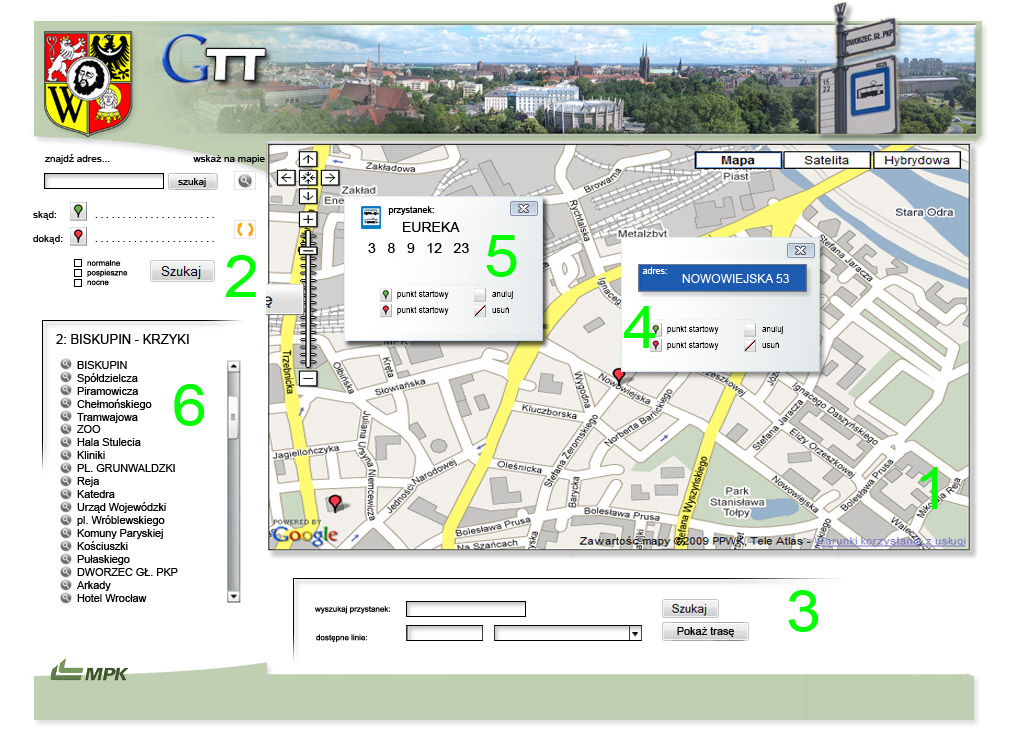
\includegraphics[width=\textwidth]{interfejs_help} 
\caption{Interfejs użytkownika \textbf{GTT}}\label{interfejs_help}
\end{figure}
 \begin{enumerate}
	\item mapa -- najistotniejszy element systemu. Dzięki mapie tak łatwo odnaleźć
	interesujące miejsca -- w końcu nie trzeba pamiętać adresu czy wręcz nazwy
	przystanku. Na mapie przedstawiane są wszelkie wyniki wyszukiwań czy to
	połączeń, czy przystanków, czy też wyświetlane są trasy wybranych linii.
   \item panel wyszukiwania połączeń -- to tutaj rozpoczyna się proces
   wyszukiwania i wybór punktów startowego i docelowego. Skorzystać można
   zarówno z wyszukiwarki jak i z pola mapowego markera umożliwającego
   zaznaczenie punktów na mapie, a następnie w otworzonym w ten sposób okienku
   wybór jako punkt startowy/docelowy. Przed wciśnięciem ,,szukaj'' warto
   zaznaczyć odpowiednie typy linii. Wyszukiwarka sama zaproponuje
   najdogodniejsze pod względem liczby przesiadek i liczby przejechanych
   przystanków połączenia oraz początkowe i końcowe przystanki najbliższe
   wybranym punktow, a całość zostanie przedstawiona na mapie.
   \item panel wyszukiwania przystanków i prezentacji trasy linii -- w tym
   miejscu można przeszukiwać bazę danych za pomocą nazw bądź fragmentów nazw
   przystanków (pasujące przystanki zostaną wyświetlone na mapie) oraz zobaczyć
   trasę wybranej linii.
   \item panel adresu -- w przypadku wyboru markera zadawania punktu
   startowego/docelowego na mapie, po kliknięciu na mapie pojawi się właśnie
   panel adresu. W nim można zobaczyć nazwę ulicy i numer (lokalizację
   wybranego punktu) oraz oznaczyć go jako początkowy/docelowy. Po kolejnym 
   kliknięciu można usunąć marker lub anulować jego oznaczenie.
   \item panel przystanku -- po wyszukaniu połaczeń, przystanków czy też
   wyświetleniu trasy linii na mapie prezentowane są markery przystanków. Po
   kliknięciu na wybrany marker wyświetlone zostanie okienko z nazwą przystanku
   oraz numerami linii, jakie na nim się zatrzymują (po klknięciu na numer
   wyświetli się tabliczka przystankowa). Można tutaj również oznaczyć
   przystanek jak początkowy/docelowy.
   \item panel prezentacji wyników -- znakomita większość informacji, które
   potrzebuje uzyskać użytkownik zostanie zaprezentowana na mapie, jednak w tym
   panelu jest możliwość dowiedzieć się jeszcze więcej, bądź też w
   alternatywny sposób dostać się do tego co potrzebne. W przypadku
   wyszukiwania połaczeń użytkownik zobaczy tutaj nazwy przystanków w kolejności
   jakie musisz pokonać oraz linie, jakimi bedzie podróżować. Jeśli uruchomione
   zostało wyszukiwanie przystanków -- w tym miejscu zostanie zaprezentowana
   ich lista, jako że najczęściej występuje wiele przystanków o tej samej
   nazwie, po kliknięciu na wybrany przystanek, podobnie jak po kliknięciu na
   niego na mapie pojawi się panel przystanku.
 \end{enumerate}
 



\end{document}